%!TEX TS-program = xelatex

\documentclass[11pt, x11names]{article}

% -- Packages ------------------------------------------------------------------

\usepackage{booktabs}
\usepackage{enumitem}
\usepackage{fontspec}
\usepackage[paperheight=25cm, paperwidth=15cm, top=0.5cm, bottom=0.5cm, left=.5cm, right=.5cm]{geometry}
\usepackage{grffile}
\usepackage{menukeys}
\usepackage{microtype}
\usepackage{minted}
\usepackage{subfig}
\usepackage{titlesec}
\usepackage{hyperref}

% -- Macros --------------------------------------------------------------------

\newcommand{\Authors}{Allan Odgaard, Brad Miller, Ciarán Walsh, Stanley Rost, Haris Skiadas, René Schwaiger}
\newcommand{\Title}{LaTeX Bundle}
\newcommand{\TitleDescription}{Documentation}
\newcommand{\Subject}{Documentation for TextMate's LaTeX Bundle }
\newcommand{\KeyWords}{TextMate, Bundle, LaTeX, XeLaTeX, LuaLaTeX, Help}

% -- Document Properties -------------------------------------------------------

\hypersetup
{
    pdftitle    = {\Title},
    pdfsubject  = {\Subject},
    pdfauthor   = {\Authors},
    pdfkeywords = {\KeyWords},
    colorlinks  = true,
    linkcolor   = black,
    anchorcolor = black,
    citecolor   = gray,
    urlcolor    = DarkOrchid4
}

\setmainfont[Mapping=tex-text]{Avenir Next}
\setsansfont[Mapping=tex-text]{Ubuntu}
\setmonofont[Scale=MatchLowercase]{Menlo}
\newfontfamily\Zapfino{Zapfino}

\setlength\parindent{0cm}
\usemintedstyle{friendly}
\pagestyle{empty}
\makeatletter \renewcommand{\@dotsep}{10000} \makeatother

\titleformat{\section}{\large\sffamily\bfseries}{}{0pt}{\thesection~·~} [{\color{DarkOrchid4}\hrule}]
\titleformat*{\subsection}{\color{DarkOrchid4}\sffamily\bfseries}
\titleformat*{\subsubsection}{\color{DarkOrchid4}\sffamily\bfseries}
\titleformat*{\paragraph}{\color{DarkOrchid4}\sffamily\bfseries}
\titleformat*{\subparagraph}{\color{DarkOrchid4}\sffamily\bfseries}

\begin{document}

% -- Text ----------------------------------------------------------------------

\begin{minipage}[t]{0.3\textwidth}
    \vspace{0cm}
    \begin{center}
        
\includegraphics[width=\textwidth]{Figures/TextMate.png}
    \end{center}
\end{minipage}
\begin{minipage}[t]{0.7\textwidth}
    \vspace{0cm}
    \begin{center}
        {\Huge\Zapfino\Title}
        \vskip 0.5cm
        {\color{DarkOrchid4}\hrule}
        \vskip 0.5cm
        {\Large\textit\TitleDescription}
    \end{center}
\end{minipage}
\vskip 1.5cm

% Table of contents without header
\makeatletter
\@starttoc{toc}
\makeatother

\section{Installing LaTeX}

To use \menu{Typeset \& View (PDF)} and other commands from the LaTeX bundle you need to install a TeX distribution. We recommend that you use \href{http://www.tug.org/mactex}{MacTeX} as it comes with a standard “no questions asked” installer.\\

MacTeX also takes care of updating your \texttt{PATH} variable. If you install another distribution you may need to \href{http://blog.macromates.com/2014/defining-a-path}{setup the path manually}.

\section{Building a LaTeX File}

\subsection{Standard Typesetting}

Most of the time you just want to typeset the currently selected file. You can accomplish this with the command \menu{Typeset \& View (PDF)}, bound to \keys{\cmd + R}. TextMate shows you, in its HTML output window, progress on the compile, as well as any errors that may occur.\\

Depending on the setting of the \menu{Keep log window open} preference, the HTML output window may stay open even after the typesetting is done. You can click on any of the errors messages in the log window. This will take you to the location of the error in the LaTeX file. Keep in mind, that LaTeX occasionally reports errors very far from where the actual problem occurs. So compile often, then you have less new text to worry about when looking for errors.

\subsection{Typesetting Multiple
Passes}

Because LaTeX processes files in a single pass, you often need to compile more than once to resolve all references. If you use citations, a glossary or other advanced LaTeX features, then you also need to use other commands such as \texttt{bibtex} and \texttt{makeindex} between runs of LaTeX. You can re-run LaTeX on the same file by clicking on the \menu{Run LaTeX} button at the bottom of the log window that appears after you invoked \menu{Typeset \& View (PDF)}. You will also find buttons in this window that allow you to run BibTeX or MakeIndex for the current file.\\

Since the process of running different typesetting programs multiple times in order to get the final document is a rather dull one we also support \href{http://ctan.org/pkg/latexmk}{latexmk}:

\begin{quote}
    Latexmk completely automates the process of generating a LaTeX document.
\end{quote}

\begin{sloppypar}
In order to tell TextMate to use \texttt{latexmk} when compiling, you have to check \menu{Use Latexmk} inside the bundle's preference window. After that you only need to invoke \menu{Typeset \& View (PDF)} once and TextMate will automatically run all necessary commands to translate your document.
\end{sloppypar}

\subsection{Using a Master File}

If you work on a large project, you probably want to use TextMate's \href{http://manual.textmate.org/projects}{support for projects}. In a larger LaTeX project, such as a book or a thesis you usually split your project in smaller files that contain one part of your document. You then include these parts in a so-called master file via the commands \texttt{\textbackslash{}input} or \texttt{\textbackslash{}include}.\\

Most of the commands of the LaTeX bundle rely on the fact that they know the location of the master file. If you do not specify the master file explicitly, then the bundle assumes that the active document is the master file. This works perfectly fine, as long as you only use one \texttt{.tex} file.\\

On the other hand, if you call a command from an included file and do not specify the master file, then the LaTeX bundle only knows about the content of the current file. This means that completion commands will only take the current file into account. E.g. \menu{Insert > Label Based on Current Word} will only list the labels in the current file. \menu{Insert > Citation Based on Current Word} might not work at all, since it only scans the current file for included bibliographies. To fix this behaviour you need to tell TextMate the location of the master file. Currently there a two possibilities to do that:

\begin{enumerate}
    \item Use the environment variable \texttt{TM\_LATEX\_MASTER}
    \item Add the \texttt{\%!TEX\ root} directive at the top of the included file
\end{enumerate}

If you specified the master file via one of these methods, then all LaTeX commands use the master file as their basis. In particular, the \menu{Typeset \& View (PDF)} and \menu{Watch Document} commands will typeset the master file, instead of whatever the currently active file is. So you can freely edit whatever chapter you are working on, and when you want to see the result you just press \keys{\cmd + R} without having to worry about switching to the master file.

\subsubsection{Using the TM\_LATEX\_MASTER Environment Variable}
\label{sec:Using_TM_LATEX_MASTER}

You can set the environment variable \texttt{TM\_LATEX\_MASTER} via a \texttt{.tm\_properties} file located at the top level folder of your project. Just create a new text file with the name \texttt{.tm\_properties} and the following content:

\begin{minted}{bash}
    TM_LATEX_MASTER = absolute_path_to_master_file
\end{minted}

You probably do not want to specify the absolute path to your master file directly, since this would mean that the location of your master file will be invalid if you move your project folder. For this purpose you can use the special variable \texttt{\$CWD}, which contains the location of the folder where the \texttt{.tm\_properties} file is located. For example, if your master file is called \texttt{Thesis.tex} and resides in the top level folder of your project, then you can use the following line to specify the location of your master file:

\begin{minted}{bash}
    TM_LATEX_MASTER = "$CWD/Thesis.tex"
\end{minted}

\subsubsection{Using the \%!TEX root Directive}
\label{sec:Using_TM_TEX_ROOT}

The LaTeX bundle supports \texttt{\%!TEX\ root} directives. You can specify the location of your master file by adding the line \texttt{\%!TEX\ root\ =\ path\_to\_master\_file} at the beginning of an included file. \texttt{path\_to\_master\_file} can be either absolute or relative.\\

For example, if your included file \texttt{Chapter\ 1.tex} is located in the folder \texttt{Chapter} inside your project folder, and your master file \texttt{Thesis.tex} is located in the top level folder of your project, then you can set the master file for \texttt{Chapter\ 1.tex} by including the following line at the top of the file \texttt{Chapter\ 1.tex}:

\begin{minted}{latex}
    %!TEX root = ../Thesis.tex
\end{minted}

You can also use the command \menu{Set Master File} to specify the master document for the current \texttt{.tex} file.

\subsection{Watching a Document}

\subsubsection{Introduction}

When you watch a LaTeX document, it is continually monitored for changes: Each time you change the content of your \texttt{.tex} file and save it, TextMate typesets it and updates the preview.

\subsubsection{Usage}

Press \keys{\ctrl + \cmd + W} to start watching a document. If the document is already being watched, you will instead be given the option to stop watching it. You can watch several documents simultaneously.\\

When you close the previewer, the associated watcher will automatically quit.

\begin{figure}[htbp]
    \begin{minipage}[t]{0.5\textwidth}
      \vspace{0cm}
      \centering
        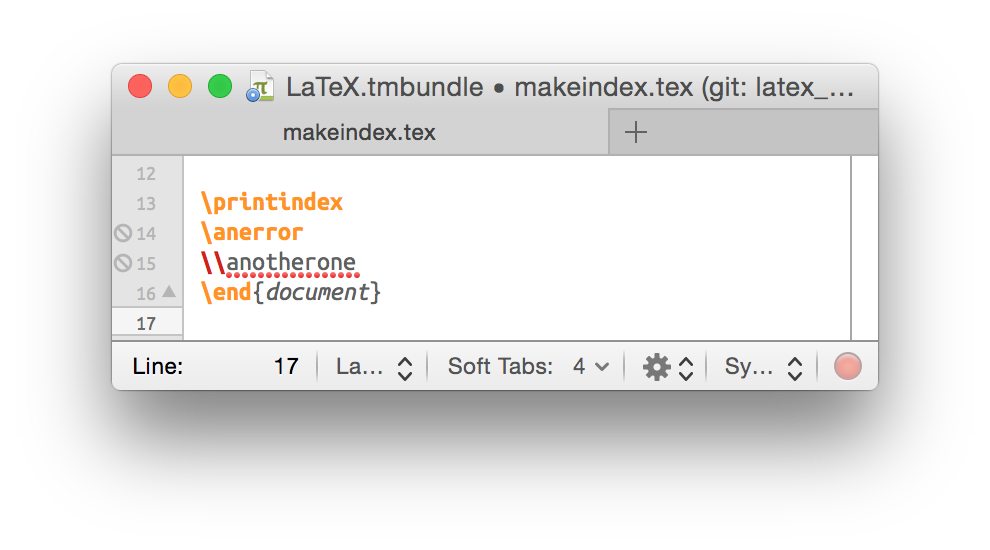
\includegraphics[width=\textwidth]{Figures/LaTeX Watch - TextMate.png}
    \end{minipage}
    \begin{minipage}[t]{0.5\textwidth}
      \vspace{0.5cm}
      \centering
        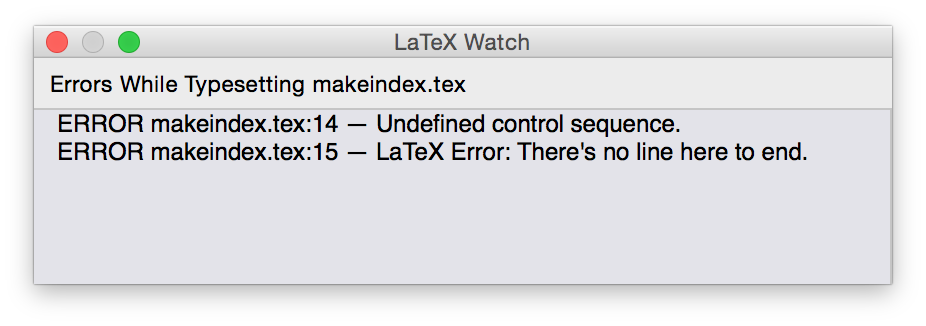
\includegraphics[width=\textwidth]{Figures/LaTeX Watch - Notification Window.png}
    \end{minipage}

    \caption{\menu{Watch Document} shows errors it detects in a floating window}
    \label{fig:LaTeX_Watch}
\end{figure}

One minor, but interesting difference between the behaviour of \menu{Stop Watching} and closing the previewer is, that in the latter case temporary files produced by LaTeX will be deleted. If you want to keep your directory clean, then you should just close the previewer after you are done. If you do not care about the auxiliary files — but instead want \menu{Watch Document} to reuse old temporary files and therefore start faster the next time, then just use \keys{\ctrl + \cmd + W} to stop monitoring the file for changes.

\section{Previewing a LaTeX File}

The \menu{Typeset \& View (PDF)} command has a second component, the “View” one. After a successful build, TextMate proceeds to show you the produced PDF file. This behaviour can be changed by toggling the checkbox \menu{Show PDF automatically} inside the bundle's preferences. If the preference item is not checked, then you can still view the file on demand by clicking the \menu{View} button at the bottom of the \menu{Typeset \& View} window.

\subsection{Default Preview}

In OS X, HTML windows can display PDF files. This is the standard behavior of the LaTeX bundle's \menu{Typeset \& View (PDF)} command. After TextMate finished the typesetting process, the window that was used to show you the building progress turns into a view of your PDF file, provided there were no errors.

\subsection{External Previewers}

You can also setup an external previewer for showing the PDF output. Focus will then switch to that previewer after TextMate finished the typesetting process. You can set the preview application inside the bundle's preferences. We recommend you use \href{http://skim-app.sourceforge.net}{Skim}, which supports SyncTeX.

\subsection{Preview Options}

Preview options are somewhat complicated depending on the viewer you choose. There are really two main cases:

\begin{enumerate}

    \item If you chose TextMate as previewer, then the \menu{Keep log window open} preference has the following effect:

    \begin{itemize}

        \item If there are no errors or warnings, the \menu{Typeset \& View} window will immediately switch to showing you the PDF file.

        \begin{sloppypar}
        \item If there are no errors but some warnings then — assuming the \menu{Keep log window open} preference is checked — you will see the warning messages. To display the PDF click on \menu{View in TextMate}. If the \menu{Keep log window open} preference is not checked, then the warning messages will be ignored and TextMate will display the PDF directly.
        \end{sloppypar}

    \end{itemize}

    \item If you use an external viewer, then the \menu{Typeset \& View} window will automatically close if there are no errors or warnings, unless the \menu{Keep log window open} preference is checked.

\end{enumerate}

\subsection{Refreshing the Viewer}

The \menu{Typeset \& View (PDF)} command uses a short Applescript to tell Skim, or the TeXShop to reload the PDF file once the typesetting is complete. This is more efficient than enabling the auto-refresh feature in the viewers, because it often takes more than one run of LaTeX before the document is really ready to view. In that case most viewers would try to reload the PDF multiple times.

\section{SyncTeX}

\href{http://mactex-wiki.tug.org/wiki/index.php/SyncTeX}{SyncTeX} allows you to easily hop back and forth between document and the generated PDF, granted you use an external previewer which supports SyncTeX.

You need to perform the following steps to enable synchronization:

\begin{enumerate}

    \item Set your viewer to \menu{Skim}. This enables you to use the\\\menu{Jump to Current Line in Viewer} command bound to \keys{\ctrl + \Alt + \cmd + O} by default.

    \item In Skim go to \menu{Preferences…}. There, choose the Preset \menu{TextMate} under the option \menu{Sync}.

    This assumes that you installed \texttt{mate} (see \menu{Preferences… > Terminal} in TextMate). After this is done, shift-command-clicking (\keys{\shift + \cmd} at a location in the PDF file (as shown in Skim) takes you to the corresponding location in TextMate.

\end{enumerate}

\textbf{Note:} The granularity of the synchronization data is generally “per paragraph”, so going from TextMate to Skim or back will generally locate just the paragraph nearest your desired position.

\section{Working With LaTeX}

This section describes the various LaTeX tasks, and how they can be accomplished with the commands provided by the bundle. Some of the commands whose behavior is clear from their name (like \menu{Format > Bold} and friends) are not included here, so you will need to traverse the submenus of the LaTeX bundle to discover them.

\subsection{Automated Typing}

Writing LaTeX often requires typing some amount of standard commands and environments. TextMate makes that a lot easier with a set of commands in the LaTeX bundle, that we'll discuss in this section.

\subsubsection{Inserting Commands and
Environments}

The LaTeX bundle contains two commands that, if you type a lot of LaTeX, will become your best friends. They are \menu{Insert > Environment Based on Current Word}, bound by default to \keys{\cmd + \textless{}}, and \menu{Insert > Command Based on Current Word}, bound by default to \keys{\cmd + \textgreater{}}. They create an environment/command based on the current word, or a default editable text in the absence of a current word. They are smart enough to understand a number of “standard” shortcuts, also called triggers. For instance, typing \texttt{thm} and then calling the \menu{Insert > Environment Based on Current Word} command creates:

\begin{minted}{latex}
    \begin{theorem}
        | ← insertion point
    \end{theorem}
\end{minted}

Similarly, typing \texttt{fig} followed by calling the \menu{Insert > Environment Based on Current Word} command creates a lot of the standard text required in a figure environment. You can further customize these commands.\\

These two commands understand a series of shortcuts, and use the current word if they do not recognize it as a shortcut. You can customize what these shortcuts are by editing the \emph{LaTeX Configuration File}. This file is originally kept in the LaTeX bundle. When you first use the \menu{Edit Configuration File} command, this file is copied to \directory{\textasciitilde{}/Library/Preferences/com.macromates.textmate.latex\_config.plist}. You can then edit this file whenever you want by executing this command, or delete it to return to the default settings.\\

This file follows the Property List Format. It consists of a top-level dictionary
with six entries:

\begin{itemize}
    \item \texttt{commands}, \texttt{environments}, \texttt{labeled\_environments}
    \item \texttt{commands\_beamer}, \texttt{environments\_beamer}, \texttt{labeled\_environments\_beamer}
\end{itemize}

\begin{sloppypar}
The versions with the word \texttt{beamer} added are the \emph{extra} shortcuts/words that TextMate recognizes in LaTeX Beamer files, \emph{in addition to the non-beamer ones}. The \texttt{commands} and \texttt{commands\_beamer} entries are dictionaries consisting of pairs, where the key is the shortcut, and the value is the text that \menu{Insert > Command Based on Current Word} inserts when it recognizes the shortcut. All inserted text, for both commands and environments, is interpreted as \href{http://manual.textmate.org/snippets.html#snippets}{Snippet}.\\
\end{sloppypar}

The four \texttt{environment} dictionaries are a bit different. They contain key-value pairs, where the key is the \emph{name} of the environment, i.e.~the text inside the braces in \texttt{\textbackslash{}begin\{\}}. The value is itself a dictionary with two entries:

\begin{description}[style=multiline, leftmargin=1.8cm]

    \item[\texttt{triggers}] is the list of shortcuts/words that will cause\\ \menu{Insert > Environment Based on Current Word} to insert the environment

    \item[\texttt{content}] is the text that TextMate inserts into the environment. If the environment is in one of the two labeled environments groups, then this text is inserted right after the closing brace in \texttt{\textbackslash{}begin\{env\}}. Otherwise, it is inserted at the beginning of the next line.

\end{description}

Another useful command is \menu{Insert > Environment Closer}, which is by default bound to \keys{\Alt + \cmd + .}. This command locates the innermost \texttt{\textbackslash{}begin\{env\}} that hasn't been closed by a corresponding \texttt{\textbackslash{}end\{env\}} and inserts the closing part. Of course, if you usually use \menu{Insert > Environment Based on Current Word}, then you probably don't need this command that often.\\

Finally, there is a command to quickly insert commands for the various symbols, called \menu{Insert > Symbol Based on Current Word}. It is bound by default to \keys{\cmd + \textbackslash{}}. It works in two stages:

\begin{itemize}

    \item First, you write down a few letters recognized by the command. The rules are basically as follows:

    \begin{itemize}

        \item Single letters are converted to greek letters

        \item Two letter combinations are converted to the various commands starting with those two letters (for instance pressing \texttt{in} would trigger commands like \texttt{\textbackslash{}int}, \texttt{\textbackslash{}inf}, \texttt{\textbackslash{}infty} etc) with a few exceptions, like \texttt{sk} for \texttt{\textbackslash{}smallskip}.

        \item Three letter combinations are converted to arrows, where the three digits signify the kind of arrow, for instance \texttt{lar} would stand for left arrows.

        \item There's a couple of exceptions to these rules. You can look at and alter the shortcuts in the LaTeX configuration file. They are located under the \texttt{symbols} key.

    \end{itemize}

    \item After you triggered the command once, pressing it again cycles through the various options. For instance, if you started with \texttt{e}, then the command cycles between \texttt{\textbackslash{}epsilon} and \texttt{\textbackslash{}varepsilon}. This is accomplished by this set of entries in the configuration file:

    \begin{minted}{properties}
    "e" = "\\epsilon";
    "epsilon" = "varepsilon";
    "varepsilon" = "epsilon";
    \end{minted}
\end{itemize}

When you create your own additions to this list, keep in mind these two simple principles: For the item that is the initial trigger, like the \texttt{"e"} above, the text must start with two backslashes. For the items used for cycling through options, it must not.

\subsubsection{List Environments}

A list of the the most commonly used LaTeX environments would certainly include the three itemize environments \texttt{itemize}, \texttt{enumerate} and \texttt{description}. The LaTeX bundle provides a few shortcuts to work with these environments. To insert one of the environments either:

\begin{enumerate}

    \begin{sloppypar}
    \item type one of the words \texttt{it}, \texttt{en} or \texttt{desc} and invoke the command \menu{Insert > Environment Based on Current Word}, or
    \end{sloppypar}

    \item type one of the words \texttt{item}, \texttt{enum} or \texttt{desc} and press \keys{\tab}.

\end{enumerate}

The first \texttt{\textbackslash{}item} is automatically inserted for you. To add a new item press \keys{\enter} and TextMate creates a new entry by inserting the command \texttt{\textbackslash{}item} in the next line. This functionality is common among most languages in TextMate that support some sort of list.\\

There is also a \menu{Lists > Itemize Lines in Selection} command, bound to \keys{\cmd + \shift + L}. It wraps the selected group of lines inside a list environment (\texttt{enumerate}, \texttt{itemize}, or \texttt{description}). Each non-blank line becomes an \texttt{\textbackslash{}item} in the environment. If the first 20 characters of every selected non-empty line contain a \texttt{:}, then the command creates a description environment. All the characters up to the \texttt{:} are placed inside brackets.

\subsubsection{Table Environments}

The command \menu{Table > Create Table} allows you to quickly inserts a table into your document. The command works both with or without a selection.\\

If you do not select any text before you invoke the command, then TextMate displays the pop-up window shown in Figure~\ref{fig:Figures_Table_-_Create_Table}. From there you can choose how many rows and columns the inserted table should have. If you check \menu{Tabular Only} — accessible via \keys{\Alt + \cmd + T} — then the command creates only a \mintinline{tex}|\tabular| environment. Otherwise the command surrounds the \mintinline{tex}|\tabular| environment with a \mintinline{tex}|\table| environment. After you hit \menu{Insert} the command places the table at the current caret position. You can then fill in the various attributes. To switch between them use the keys \keys{\tab} and \keys{\shift + \tab}.

\begin{figure}[H]
  \centering
    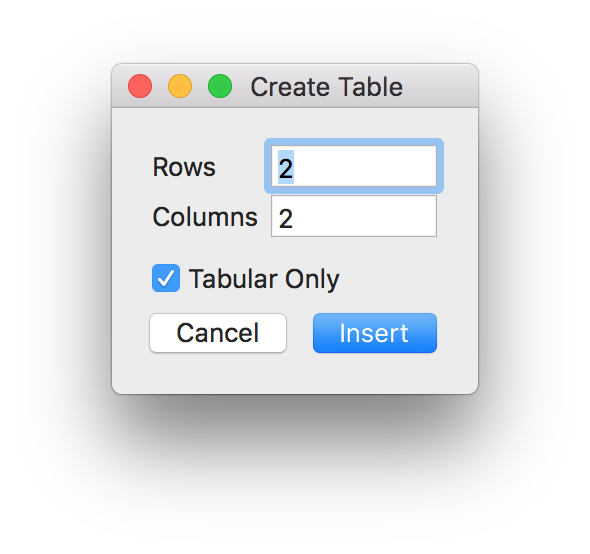
\includegraphics[width=.5\textwidth]{Figures/Table - Create Table.png}
  \caption{Graphical User Interface for the command “Create Table”}
  \label{fig:Figures_Table_-_Create_Table}
\end{figure}

If you select text before you invoke the command, then use the following format:

\begin{verbatim}
    [rows] columns [t]
\end{verbatim}

The format specification above states that you typically write down the number of rows, then the number of columns and then optionally add the character \texttt{t}, if you only want to create a tabular environment. The number of rows is optional. If you do not specify it, then TextMate will create a table with two rows. We provide two examples, which should help you understand the interface. The text above the example shows the selection. After that we show the inserted LaTeX code, followed by the rendering of the translated code.

\paragraph{Selected Text: \menu{2 3}}

\inputminted[frame=lines]{tex}{TeX/Table_2_3.tex}
\begin{table}[htb!]
  \caption{Caption}
  \label{table:label}
  \centering
  \begin{tabular}{ccc}
    \toprule
    \textbf{Header 1} & \textbf{Header 2} & \textbf{Header 3}\\
    \midrule
                 r2c1 &              r2c2 &              r2c3\\
    \bottomrule
  \end{tabular}
\end{table}


\paragraph{Selected Text: \menu{3 4 t}}

\inputminted[frame=lines]{tex}{TeX/Table_3_4_t.tex}
\begin{tabular}{llll}
  r1c1 & r1c2 & r1c3 & r1c4\\
  r2c1 & r2c2 & r2c3 & r2c4\\
  r3c1 & r3c2 & r3c3 & r3c4\\
\end{tabular}


\subsubsection{Wrapping Text}

Often one wants to enclose the currently selected text in an environment, or a command. The LaTeX bundle offers a list of \menu{Wrap\ Selection\ In} commands for all tastes. Here they are:

\begin{description}

    \item[\menu{Wrap Selection in > Command}]~\hfill~\keys{\ctrl + \shift + W}\\

    This command wraps the selected text in the command \texttt{\textbackslash{}emph\{\}}. To change the environment press the tab key once and write down the name of the command you want. If you did not select any text before invoking the command, then you can press tab once again to insert a text into the empty environment you just created.

    \item[\menu{Wrap Selection in > Environment}]~\hfill~\keys{\ctrl + \shift + \cmd + W}\\

    This command wraps the selected text in an environment. It also works without a selection.

    \item[\menu{Wrap Selection in > Double Quotes}]~\hfill~\keys{\ctrl + \texttt{`}}\\

    Wraps the currently selected text in LaTeX double quotes,\\
    i.e. \texttt{``selection here''}.

    \item[\menu{Wrap Selection in > left…right}]~\hfill~\keys{\ctrl + \shift + L}\\

    Wraps the currently selected text in the \texttt{\textbackslash{}left-\textbackslash{}right} pair. I.e. if you select \texttt{(text\ here)} and invoke the command, then TextMate replaces it with \texttt{\textbackslash{}left(text\ here\textbackslash{}right)}.

    \item[\menu{Wrap Selection in > Display Math}]~\hfill~\keys{\ctrl + \shift + M}\\

    This command wraps the selection between the text \texttt{\textbackslash{}{[}} and \texttt{\textbackslash{}{]}}.

    \item[\menu{Wrap Selection in > Math Mode}]~\hfill~\keys{\ctrl + \shift + M}\\

    This command inserts \texttt{\textbackslash{}(} before, and \texttt{\textbackslash{})} after the selection.

\end{description}

\subsection{Completion}

The LaTeX bundle adds the following words to the list of completions (accessed through \keys{\esc}): corollary, definition, description, enumerate, equation, itemize, lemma, proof, proposition and verbatim.

\subsubsection{Commands}

We already talked about how you can quickly create a command with \menu{Insert > Command Based on Current Word}. You can also complete a partial typed command with \menu{Insert > Command Completion}. Just write down the first characters of your word, e.g. \mintinline{tex}|\table|, and press \keys{\Alt + \esc}. TextMate will then display a menu with possible completions consisting of predefined commands and commands from your current master file.

\subsubsection{Citations and References}

The LaTeX bundle overrides the standard completion behavior when the caret is inside a \texttt{\textbackslash{}cite\{\}} or \texttt{\textbackslash{}ref\{\}} block. It also overrides the completion behaviour for other equivalent commands like \texttt{eqref}, \texttt{vref}, \texttt{prettyref}, \texttt{citeauthor} etc.\\

If the LaTeX command expects a bibliography key, then pressing \keys{\esc} inside the braces offers completion with respect to all cite keys. This is accomplished by scanning all bib files included in the current master file. For instance, if the caret is right before the closing brace in \texttt{\textbackslash{}cite\{Ka\}}, then pressing \keys{\esc} will cycle trough all bibliography keys starting with \texttt{Ka}.\\

If the LaTeX command expects a label key, pressing \keys{\esc} inside the braces of the command will cycle trough all labels of the current master document. You can narrow the search down by writing part of the label key before you hit \keys{\esc}. This is especially useful if you use a prefix that specifies the type of the reference in your labels. For example, if you prefix each label of a theorem with \texttt{thm:} — i.e.~all theorem labels have the form \texttt{thm:labelname}, then pressing \keys{\esc} when the caret is right before the closing brace in \texttt{\textbackslash{}ref\{thm:\}} will offer as completion options all labels referencing theorems.\\

If there are many matching completions, it is often more convenient to use the pull-down-list versions of the commands:

\begin{itemize}
    \item \menu{Insert > Label Based on Current Word}
    \item \menu{Insert > Citation Based on Current Word}
    \item \menu{Insert > Citation (Ref-TeX Style)}
\end{itemize}

You can trigger them by pressing \keys{\Alt + \esc}.

\begin{figure}[h]
  \centering
    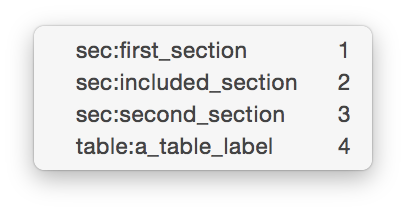
\includegraphics[width=0.3\textwidth]{Figures/Label Completion}
  \caption{\menu{Insert > Label Based on Current Word} in action}
  \label{fig:Figures_Label_Completion}
\end{figure}

Both the label and bibliography completion commands also work outside of a \texttt{\textbackslash{}ref\{\}} or \texttt{\textbackslash{}cite\{\}} block. They will insert the \texttt{\textbackslash{}ref} or \texttt{\textbackslash{}cite} for you, if you call them outside of the aforementioned blocks. Here are a two examples of the usual use cases for the commands:

\begin{itemize}

    \item You want to insert a citation after the word \texttt{example} and you do not know anything about the cite key, author or title. Just insert a \texttt{\textasciitilde{}} after the word \texttt{example}, press \keys{\Alt + \esc} and select \menu{Citation Based on Current Word…}. TextMate will show you a list of all citations. Just select the one you want via the keyboard or mouse. If we assume that the item you chose has the citekey \texttt{theKey}, then TextMate will replace \texttt{example\textasciitilde{}} with \texttt{example\textasciitilde{}\textbackslash{}cite\{theKey\}}.

    \begin{sloppypar}
    \item You want to insert a citation after the word \texttt{example\textasciitilde{}} and you know that the title of the document you want to cite contains the word \texttt{important}. Just add \texttt{important} after \texttt{example\textasciitilde{}}, press \keys{\Alt + \esc} and select \menu{Citation Based on Current Word…}. TextMate will now show you a list of all citations that contain the word important somewhere in their title, citekey, or authors tag. If we again assume that the item you chose has the citekey \texttt{theKey}, then TextMate will replace \texttt{example\textasciitilde{}important} with \texttt{example\textasciitilde{}\textbackslash{}cite\{theKey\}}.
    \end{sloppypar}

\end{itemize}

\begin{figure}[h]
  \centering
    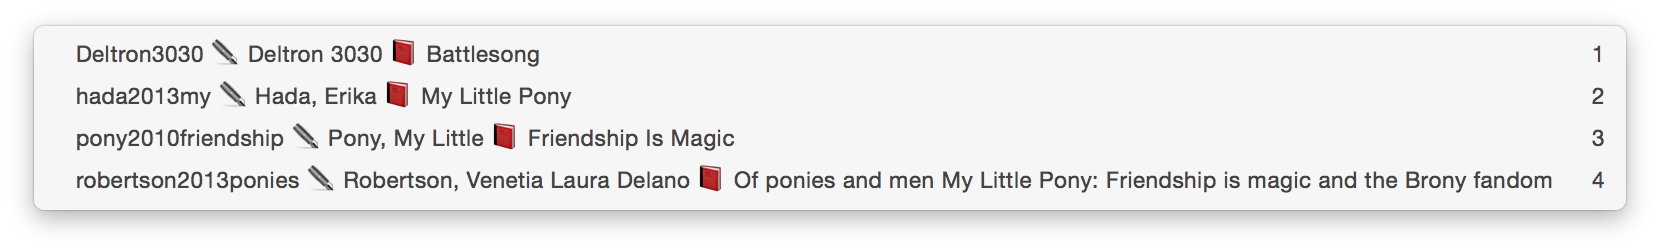
\includegraphics[width=\textwidth]{Figures/Citation Completion.png}
  \caption{\menu{Insert > Citation Based on Current Word} in action}
  \label{fig:Figures_Citation_Completion}
\end{figure}

One minor but interesting feature of the completion commands is, that they interpret the current word/selection as regular expression. For example, if you selected the text \texttt{foo\textbar{}bar} and press \keys{\Alt + \esc} then the completion commands will narrow down the completion list to labels/citations that contain one of the words \texttt{foo} or \texttt{bar}.

\subsection{Advanced Tasks}

\subsubsection{LaTeX Beamer}

The LaTeX bundle contains special supports for the \href{https://bitbucket.org/rivanvx/beamer/wiki/Home}{Beamer document class}:

\menu{Insert Environment} and \menu{Insert Command} understand more shortcuts, and also behave intelligently with respect to other shortcuts, adding overlay specifications where appropriate. The same goes for the \menu{Lists > New Item} command.\\

In order for all this to work, make sure that the language for the document is set to \menu{LaTeX Beamer} (\keys{\ctrl + \shift + \Alt + B}).

\subsubsection{Drag and Drop}

There are three key drag and drop commands in LaTeX:

\begin{itemize}

    \item You can drag an image file in to the document and have it surrounded by a complete figure environment. Using the modifier key \keys{\Alt} while dragging inserts the image surrounded by a \texttt{center} environment. If you use the modifier \keys{\shift}, then TextMate only inserts the \texttt{\textbackslash{}includegraphics} line.

    \item You can drag in another \texttt{.tex} file into your document. TextMate will then insert a \texttt{\textbackslash{}include} command that references the dropped file. To use a \texttt{\textbackslash{}input} command instead use the modifier key \keys{\Alt}.

    \item If you drop a source code file into your document, then TextMate creates a new \mintinline{tex}|listing| command referencing the dropped file. Said command is part of the \href{http://ctan.org/pkg/minted}{minted} package. To successfully translate the resulting document include \mintinline{tex}|minted| and install the various package dependencies. Do not forget to specify the option \texttt{-shell-escape} (see section “\nameref{sec:preferences}”), otherwise the translation will fail.\\

    If you want to include dropped code via the command \mintinline{tex}|lstinputlisting|, use the modifier key \keys{\shift}. To translate the resulting document you need the \texttt{listings} package. Make sure that you include it via \mintinline{tex}|\usepackage{listings}|.

\end{itemize}

\subsubsection{Templates}

The LaTeX bundle offers a simple template system. We provides a few sample files. If you want to use your own templates, then create the directory \directory{\textasciitilde{}/Library/Application\ Support/LaTeX/Templates}. In there you can put any \texttt{.tex} files you like. We also support snippet syntax in template files. To tell TextMate that it should insert the code using snippet syntax add the following line at the top of the template:

\begin{minted}{latex}
    %!TEX style = snippet
\end{minted}

\begin{figure}[h]
  \centering
    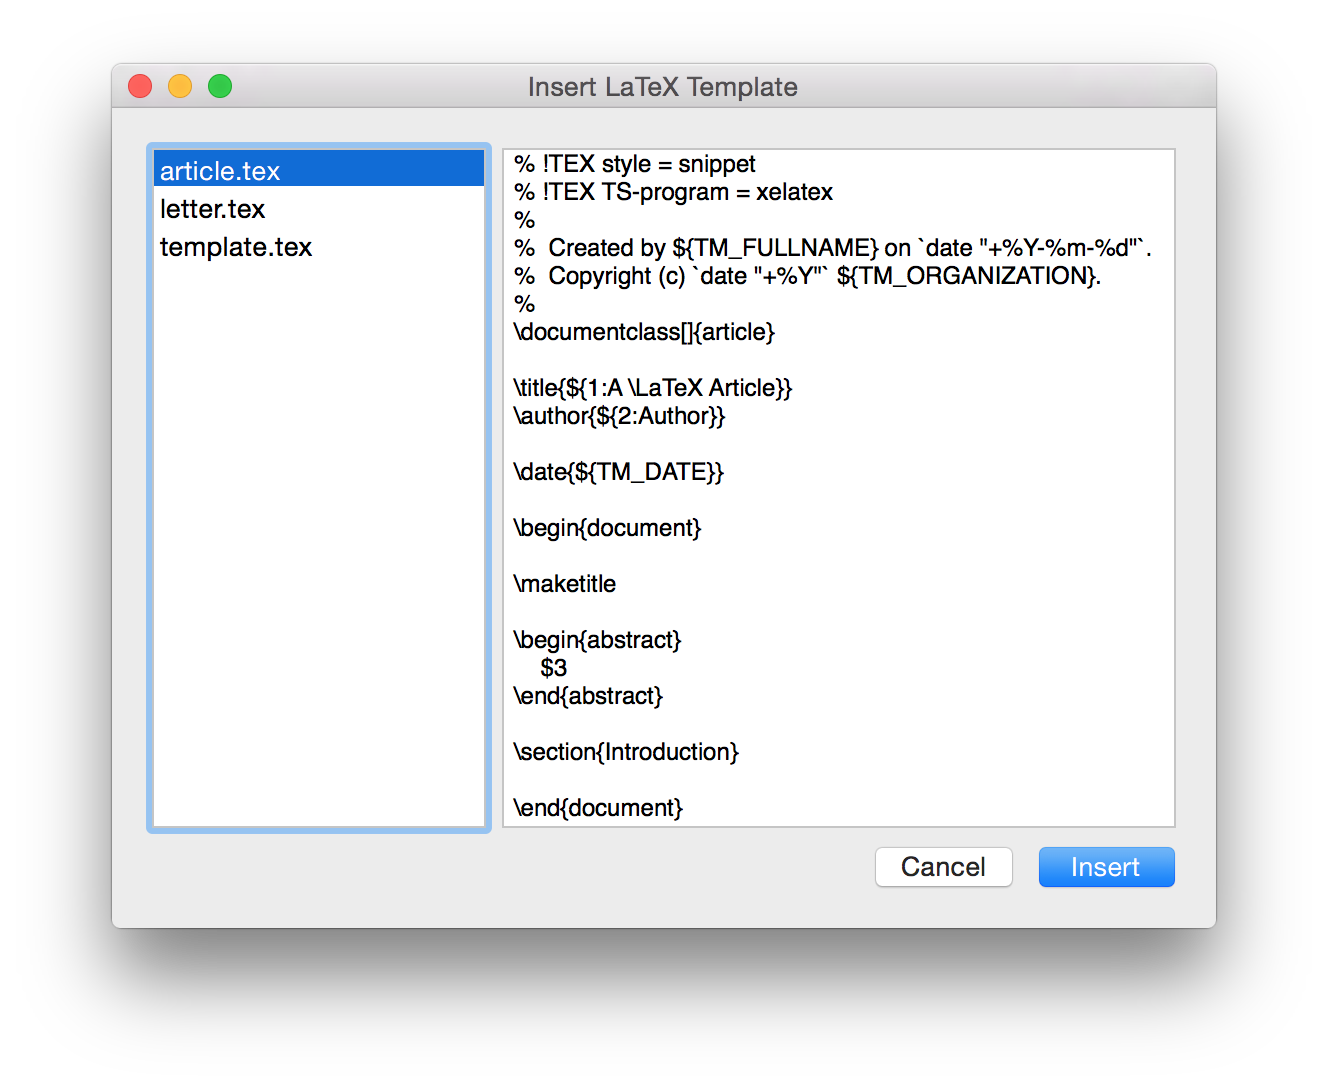
\includegraphics[width=.8\textwidth]{Figures/Template Chooser.png}
  \caption{\menu{Insert > LaTeX Template} lets you insert LaTeX code into your document}
  \label{fig:Figures_Template_Chooser}
\end{figure}

To insert a template use the command \menu{Insert > LaTeX Template}. The command will show you a window containing a list of all available templates. Select one of these files via the button \menu{Insert}. TextMate will paste the contents of that file at the cursor's location.\\

A typical workflow for the template system looks like this:

\begin{itemize}
    \item Create new file — \keys{\cmd + N}
    \item Set Language to LaTeX — \keys{\shift + \ctrl + \cmd + L}
    \item Type \texttt{temp} and press \keys{\tab}
    \item Use arrows/keys/mouse to select the template file and press \keys{\return}
    \item Start working on your document
\end{itemize}

\section{Preferences}
\label{sec:preferences}

\subsection{Global Preferences}

To show the Preferences panel for LaTeX select the command \menu{Preferences…} or press \keys{\Alt + \cmd + ,} in any LaTeX document. The Preferences window allows you to set options concerning typesetting and viewing.

\begin{figure}[h]
  \centering
    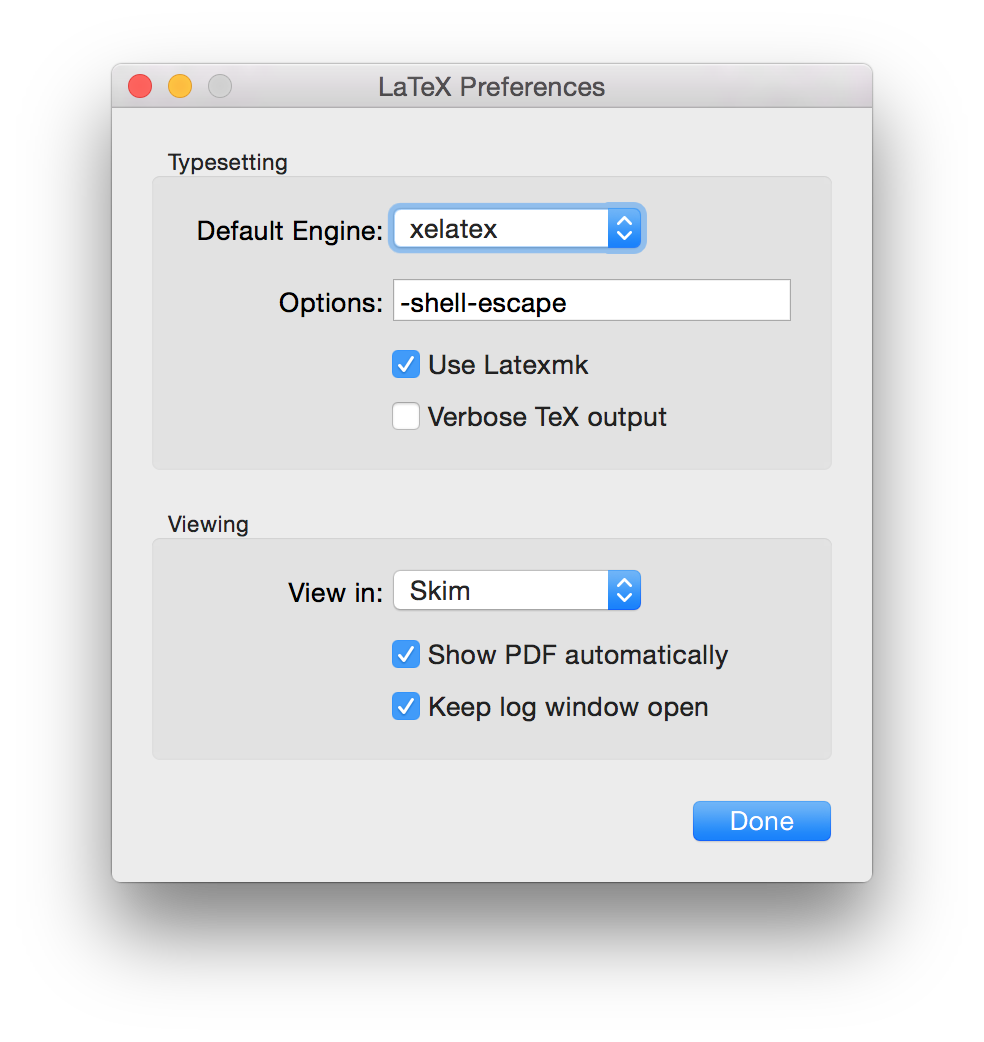
\includegraphics[width=.8\textwidth]{Figures/Preferences}
  \caption{The settings window of the LaTeX bundle}
  \label{fig:Figures_Preferences}
\end{figure}

The following typesetting options are available:

\begin{description}[style=multiline, leftmargin=4cm]

    \item[Default Engine] Choose your preferred typesetting engine from the dropdown list. You can override the default engine by using the \texttt{\%!TEX\ TS-program\ =} directive in your source file (see “\nameref{sec:Local_Preferences}”).

    \textbf{Note:} \menu{Typeset \& View (PDF)} will override the typesetting engine if it detects a package in your source file that is not compatible with the default engine. This only happens if you do not specify the engine via \texttt{\%!TEX\ TS-program}.

    \item[Options] If you have specific options that you want to pass to the engine, then you can set them here. If you have options that are specific to a single file, then use the \texttt{\%!TEX\ TS-options\ =} directive at the top of your source file.

    \textbf{Note:} \menu{Watch Document} currently does not support the \texttt{\%!TEX\ TS-options} directive.

    \item[Use Latexmk] TextMate supports the popular \texttt{latexmk} script which automatically runs \texttt{latex}, \texttt{bibtex}, \texttt{makeindex} and other commands as many times as needed to resolve all cross references and citations in your file. To use \texttt{latexmk} just check this box.

    \textbf{Note:} \menu{Watch Document} always uses \texttt{latexmk} to translate a LaTeX document, regardless of this setting.

    \item[Verbose TeX output] If you want to see the raw log file produced by LaTeX in the \menu{Run \& View (PDF)} window, then check this box.

\end{description}

You can set the following viewing options:

\begin{description}[style=multiline, leftmargin=5cm]

    \item[View in] Select one of the supported viewers. We recommend that you install and use \href{http://skim-app.sourceforge.net}{Skim}.

    \item[Show PDF automatically] If you want that the viewer starts automatically after the typesetting is done, check this box.

    \item[Keep log window open] If you want the log window to stay open — so you can check error and warning messages — check this box.

\end{description}

If you use TextMate as viewer — instead of an external viewer like Skim, then you should keep the following in mind: \menu{Show PDF automatically} will not show the PDF file if there are any errors or warnings if \menu{Keep log window open} is checked. If the option is not checked, then the PDF automatically replaces the log assuming there are no errors.

\subsection{Local Preferences}
\label{sec:Local_Preferences}

There are three options that you can set on a per file basis. As mentioned above these options will override the preferences that you set using the preferences interface.\\

You can set these “local options” via the \texttt{\%!TEX} directives \texttt{root}, \texttt{TS-program} and \texttt{TS-options}:

\begin{description}[style=multiline, leftmargin=2.4cm]

    \item[\texttt{root}] This option allows you to set a master file. More information about this directive is available in the section “\nameref{sec:Using_TM_TEX_ROOT}”.

    \item[\texttt{TS-program}] To override the typesetting engine for a particular file you can use this directive. For example, to use the engine \texttt{xelatex} for a specific document, add the line \texttt{\%!TEX\ TS-program\ =\ xelatex} at the beginning of the master file.
    \emph\emph{{}}
    \item[\texttt{TS-options}] You can add file specific (engine) options via this directive.

    \textbf{Note:} Whatever options you choose they will be used in the addition to the default options \texttt{-interaction=nonstopmode} and \texttt{-file-line-error-style}.

\end{description}

\subsection{Environment Variables}

The LaTeX bundle supports environment variables that let you modify the behaviour of certain commands. You can set this variables either via a \href{http://blog.macromates.com/2011/git-style-configuration}{.tm\_properties} file or in the Preferences of TextMater under the tab \menu{Variables}.

\begin{figure}[h]
  \centering
    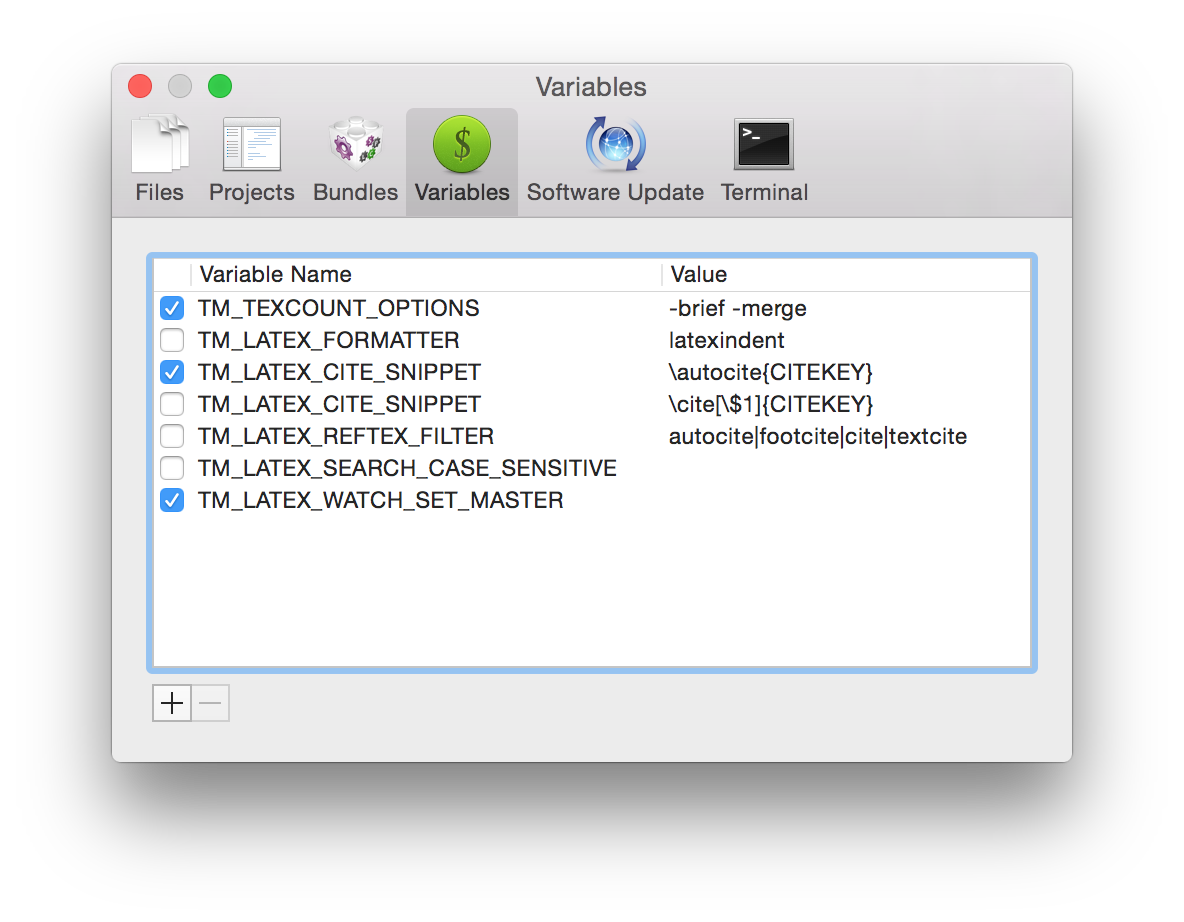
\includegraphics[width=.8\textwidth]{Figures/TextMate Preferences - Variables.png}
  \caption{Set environment variables under \menu{TextMate > Preferences… > Variables}}
  \label{fig:Figures_TextMate_Preferences_-_Variables}
\end{figure}

\begin{description}

    \item[\texttt{TM\_LATEX\_CITE\_SNIPPET}]~\\

    \begin{sloppypar}
    You can change the default substitution text used by \menu{Insert > Citation Based on Current Word} — \verb|\cite{CITEKEY}| — via this variable. Every occurrence of \texttt{CITKEY} specified via this variable will be replaced with the chosen citekey. This variable support snippet syntax.
    \end{sloppypar}

    \item[\texttt{TM\_LATEX\_FORMATTER}]~\\

    This variable lets you specify the program used in the command \menu{Tidy}. Currently the only option besides the default formatter \href{http://bfc.sfsu.edu/cgi-bin/hsu.pl?LaTeX_Tidy}{LaTeX\_Tidy} is \href{https://github.com/cmhughes/latexindent.pl}{latexindent}.

    \item[\texttt{TM\_LATEX\_REFTEX\_FILTER}]~\\

    This is a regular expression that lets you filter the entries displayed by \menu{Insert > Citation (Ref-TeX Style)}. Figure~\ref{fig:TM_LATEX_REFTEX_FILTER} shows you the output of the command without this variable on the left, and with the variable set to
    \begin{minted}{bash}
        autocite|footcite|cite|textcite
    \end{minted}
    on the right.

    \begin{figure}[htbp]
        \begin{minipage}[t]{0.5\textwidth}
          \vspace{0cm}
          \centering
            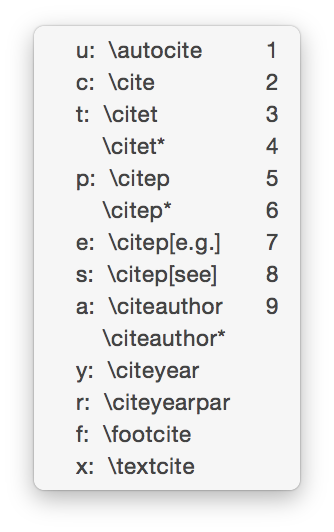
\includegraphics[width=0.5\textwidth]{Figures/Citation Completion - Without Ref-TeX Filter}
        \end{minipage}
        \begin{minipage}[t]{0.5\textwidth}
          \vspace{0cm}
          \centering
            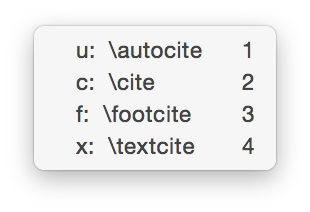
\includegraphics[width=0.5\textwidth]{Figures/Citation Completion - With Ref-TeX Filter}
        \end{minipage}

        \caption{\texttt{\texttt{TM\_LATEX\_REFTEX\_FILTER}} lets you filter the menu entries of \menu{Insert > Citation (Ref-TeX Style)}}
        \label{fig:TM_LATEX_REFTEX_FILTER}
    \end{figure}

    \item[\texttt{TM\_LATEX\_SEARCH\_CASE\_SENSITIVE}]~\\

    The commands:

    \begin{itemize}
        \item \menu{Insert > Citation Based on Current Word}
        \item \menu{Insert > Citation (Ref-TeX Style)}
        \item \menu{Insert > Label Based on Current Word}
    \end{itemize}

    interpret the current word/selection as case-insensitive regular expression by default. They use this expression to filter the possible entries they display. To interpret the selection instead as case sensitive expression set this variable (to any value you like).

    \item[\texttt{TM\_LATEX\_WATCH\_SET\_MASTER}]~\\

    If you set this variable — you can use any value you like — then \menu{Watch Document} sets \texttt{TM\_LATEX\_MASTER} to the path of the watched file. For this purpose the command creates a \texttt{.tm\_properties} file in the folder of the watched file. This works only if there is no such file in the folder already. If your project folder already contains a \texttt{.tm\_properties} file, then you can of course still set the master file yourself. Just define the \texttt{TM\_LATEX\_MASTER} variable. For a description of how to do that, please just consult the section “\nameref{sec:Using_TM_LATEX_MASTER}”.

    \item[\texttt{TM\_TEXCOUNT\_OPTIONS}]~\\

    \begin{sloppypar}
    This environment variable specifies additional options for the program \texttt{texcount}. The LaTeX bundle uses this tool to print statistics about the word count of the current master file. Figure~\ref{fig:TeXcount} shows the output with the default options \texttt{-nocol -utf8 -inc} on the left, and the \emph{additional} options \texttt{-brief -merge} on the right.
    \end{sloppypar}

    \begin{figure}[htbp]
        \begin{minipage}[t]{0.5\textwidth}
          \vspace{0cm}
          \centering
            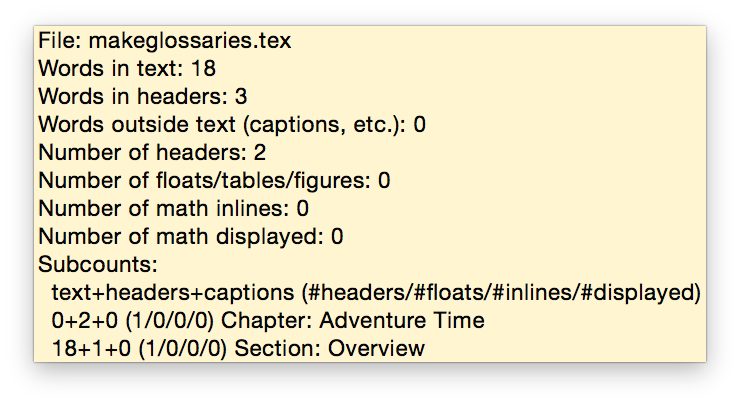
\includegraphics[width=\textwidth]{Figures/TeXcount - Default Options.png}
        \end{minipage}
        \begin{minipage}[t]{0.5\textwidth}
          \vspace{0cm}
          \centering
            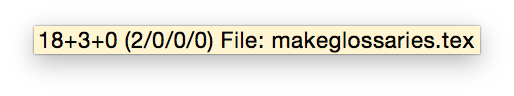
\includegraphics[width=\textwidth]{Figures/TeXcount - Custom Options}
        \end{minipage}

        \caption{\texttt{TM\_TEXCOUNT\_OPTIONS} lets you change the output of \menu{Project Management > TeXcount}}
        \label{fig:TeXcount}
    \end{figure}

\end{description}

\section{Credits}

There were at least two or possibly three versions of a LaTeX bundle floating around in the early days of TextMate by: Normand Mousseau, Gaetan Le Guelvouit and Andrew Ellis. At some point — January 2005 — Eric Hsu pulled together the threads into one package. From then on there have been contributions by Sune Foldager, Brad Miller, Allan Odgaard, Jeroen van der Ham, Robin Houston, Haris Skiadas and many other \href{https://github.com/textmate/latex.tmbundle/graphs/contributors}{contributors}.\\

Happy LaTeXing!

\end{document}
